\documentclass{article}
\usepackage[utf8]{inputenc}
\usepackage{graphicx}
\usepackage{kotex}

\title{EW final}
\author{201824501 손재성}
\date{December 2022}

\begin{document}
\maketitle
\section{8. Table, Image, and \LaTeX}
\subsection {표}

\begin{table}[ht!]
\centering
\caption{Table template for EW}
\label{t1}
\begin{tabular}{|c|c|c|c|}
\noalign{\smallskip}\noalign{\smallskip}\hline
& column1 & column2 & column3 \\
\hline 
row1 & - & - & - \\
\hline
row2 & - & - & - \\
\hline
row3 & - & - & - \\
\hline
\end{tabular}
\end{table}

\begin{table}[ht!]
\centering
\caption{Table template 2 for EW}
\label{t2}
\begin{tabular}{c|ccc}
\noalign{\smallskip}\noalign{\smallskip}\hline\hline
& column1 & column2 & column3  \\
\hline
row1 & - & - & - \\
\hline
row2 & - & - & - \\
\hline
row3 & - & - & - \\
\hline
\hline
\end{tabular}
\end{table}

\subsection{이미지}

\textbackslash usepackage\{graphicx\}를 사용해야 한다.
\begin{figure}[ht!]
\centering
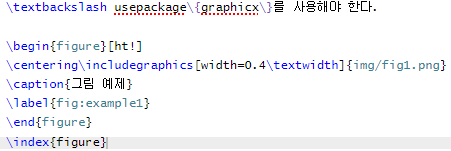
\includegraphics[width=0.4\textwidth]{img/fig1.png}
\caption{그림 예제}
\label{fig:example1}
\end{figure}
\index{figure}

\subsection{인용}
문헌 목록은 thebibliography환경으로 만든다.

\textbackslash bibitem[label]{marker} 명령으로 시작하여 입력한다.

marker는 문서 내에서 이 도서나 논문 등의 문헌을 인용하는데 다음과 같이 사용된다.

\textbackslash cite{marker}

example~\cite{ex1} is thebibliography example


\subsection{정형 데이터}
\begin{itemize}
    \item 표 형태로 저장이 가능하고, 모든 행들이 같은 구조(같은 속성)를 가진 데이터, 즉 형태가 있는 데이터이다.
    \begin{itemize}
        \item 정형 데이터는 쉽게 저장하고, 정돈하고, 검색하고, 재정렬해서 다른 정형 데이터와 결합할 수 있다.
        \item 정형 데이터는 데이터 과학 분석을 하기가 비교적 쉽다. 분석 기록으로 변환 및 적용하기 적합한 포맷으로 정의되어 있기 때문이다.
    \end{itemize}
    \item 이미지 등은 비정형 데이터이다.
\end{itemize}
\subsubsection{데이터를 설명하는 몇가지 용어}
\begin{itemize}
    \item 변수(variable) : 인구, 한국인, 외국인, 세대당 인구, 65세 이상 고령자 \ldots
    \item 값(value) : 4378, 3497 \ldots
    \item 관측치(Obserbation) : 값을 측정한 단위, 시군구 \ldots
\end{itemize}
\subsubsection{깔끔한 데이터 - tidy data}
\begin{itemize}
    \item 우리는 데이터 분석을 수행하면서 다양한 데이터 변환 작업을 수행하게 된다. 이는 데이터가 원래 특정 분석을 염두에 두고 만들어지는 경우가 거의 없기 때문이며, 사실 애초 데이터 설계를 할 때 분석 목적을 알기도 불가능하다는 게 가장 큰 원인이 아닐까 한다. 이런 연유로 전체 데이터 분석 작업에서 70\%혹은 80\% 이상이 이런 데이터 변환 및 전처리 작업에서 소모된다.
    \item 지저분한 데이터의 경우 treatmenta, treatmentb등과 같이 속성의 이름이 없다. 이는 해당 데이터가 데이터인지 속성인지 햇갈리게 한다.
    \item 지저분한 데이터의 특징은 아래와 같다.
    \begin{itemize}
        \item 열 이름이 변수 이름이 아니고 값인 경우
        \item 같은 표에 다양한 관측 단위가 있는 경우
        \item 하나의 열에 여러 값이 들어 있는 경우
        \item 변수가 행과 열에 모두 포함되어 있는 경우
        \item 하나의 관측 단위가 여러 파일로 나누어져 있는 경우
    \end{itemize}
    \item 깔끔한 데이터의 경우 아래와 같은 특징을 가진다.
    \begin{itemize}
        \item 각 변수는 개별의 열로 존재한다.
        \item 각 관측치는 행을 구성한다.
        \item 각 표는 단 하나의 관측기준에 의해서 조직된 데이터를 저장한다.
        \item 만약 여러개의 표가 존재한다면, 적어도 하나 이상의 열이 공유되어야 한다.
    \end{itemize}
\end{itemize}

\subsection{8장 요약}
\begin{itemize}
    \item 각 표는 단 하나의 관측기준에 의해서 조작된 데이터를 저장한다.
    \item 배치 순서를 의식한다.
    \item 각 변수는 개별의 열로 존재한다.
    \item 각 관측치는 행을 구성한다.
    \item 숫자표는 자리 수를 맞춰서 오른쪽으로 정렬한다.
    \item 수치는 가로보다 세로로 비교한다.
    \item 여러개의 표가 존재한다면, 적어도 하나이상의 열이 공유되어야 한다.
\end{itemize}

\begin{thebibliography}{99}
    \bibitem{ex1} blablabla: blablablabla (2022)
\end{thebibliography}

\section{9. Cover letter, Resume, Portfolio}
\subsection{자기소개서, Cover letter}
\begin{itemize}
    \item 인사 담당자 등에게 이력서와 함께 동봉하여 보내는 편지, 한국에서는 주로 자기소개서를 의미한다.
    \begin{itemize}
        \item 커버 레터는 국문 자기소개서의 축약본이라고 보면 된다. 인사 담당자는 커버 레터를 보고 지원자의 이력서를 읽을지 판단한다.~\cite{c1} 
        \item 외국계 기업에 지원할 때는 커버레터 라는 것을 써야 한다. 커버 레터에는 자신의 이력서와 자기소개서가 엉뚱한 부서로 가는 일이 없도록 어느 부서에 지원하는 것이고, 어느 시기에 지원하는 것인지 등을 구체적으로 기입해야 한다.~\cite{c2}
    \end{itemize}
    \item 자기소개서의 중요성
    \begin{itemize}
        \item 이력서만으로 모든 것을 확인할 수 없기 때문에 면접관이 지원자에게 직무/학업 관련 질문을 하는데 활용하는 핵심적인 자료
        \item 명확하게 작성하는 것이 중요하다.
        \item 직무/학업 연결성이 높아야 한다.
        \item 쓸데없는 소리하지말고 왜 이 직업을 선택했으며 왜 이런 선택을 했는지 등등 직무관련 질문을 유도하기 위해 작성해야 한다.
        \item 자연스러운 흐름을 활용한다.
        \item 자신이 무엇을 원하는지, 무엇을 잘하는지에 대한 객관적인 관점이 필요하다.
        \item 해당 관점을 하나의 흐름으로 연결하는 것이 중요하다.
        \item 반드시 작성해 봐야 한다.
    \end{itemize}
\end{itemize}
\subsection{이력서, Resume}
\begin{itemize}
    \item 자신의 이력 사항을 기입한 것이다.
    \item 하나로 여러 곳에 제출할 수 있다.
    \item 주로 조직이나 특정 집단에 합류하기 위한 목적으로 자신의 정보를 기록/배포하기 위한 목적으로 작성한다.
    \item 자신의 능력과 경험을 체계적으로 정리한 문서이다.
    \item 사실상 공식적인 문서로 취급한다.
    \item 자기 자신이 작성하는 것이 주된 특징이다.
    \item 매우 dry하게 작성한다.
\end{itemize}
\subsection{포트폴리오, portfolio}
\begin{itemize}
    \item 포트폺리오는 서류가방, 작품집, 유가 증권 보유 알림표 등의 사전적 뜻을 가진다.
    \item 일반적으로 심사 목적으로 작품이나 성과 등의 경력을 정리한 자료집이라는 의미로 사용한다.
    \item 자신의 이력, 경력 또는 실력 등을 확인할 수 있도록 과거에 만든 작품이나 관련 내용 등을 모아 놓은 것으로 실기와 관련된 경력증명서이다.
    \item 예술 및 기술 분야에서 자신의 작업물을 타인에게 증명하기 위해 필수적이다.
    \item 일반적으로 바인더, 스크랩북 등을 이용한다. 현대에는 CD-ROM및 블로그, 개인 홈페이지를 이용한다.
    \item 현재의 포트폴리오는 의미가 확장되어, 여러 분야에서 자신이 만들었던 결과물을 모아둔 경력 증명서 전체를 뜻하는 의미로 일반화되었다.
    \item 예를 들어, 게임 개발에 참여했던 사람들은 소속된 집단의 이름만 가지고 어떤 작업을 했는지 쉽게 파악이 힘들다.
    \item 프리랜서로 일하는 경우 역시 경험과 경력을 가늠하기가 힘들다.
    \item 배치 순서가 중요하다. 가장 자신있는 것일수록 앞쪽에 둔다.
    \item 보통은 졸업과제 정도가 포토폴리오 맨 앞에 온다. + 수상 관련 포토폴리오
\end{itemize}
\subsection{우리들의 이력서}
\begin{itemize}
    \item 국문 이력서
    \begin{itemize}
        \item 한국에서 사용하는 대표적인 이력서는 현재 대부분의 조직에서 활용하고 있지 않다.
        \item 이력서에 과도한 개인정보를 요구하고 있으며, 해당 이력서를 통해서 지원자의 역량을 파악하기 쉽지 않다.
    \end{itemize}
    \item 영문 이력서
    \begin{itemize}
        \item 일반적인 이력서 작성 순서는 아래와 같다
        \item 머리말(heading) - 목적(Objective) - 학력(Education) - 경험(Experience) - 추가정보
    \end{itemize}
    \item 이력서를 작성하는 이유
    \begin{itemize}
        \item 이력서는 면접 기회를 얻기 위한 문서이다.
        \item 담당자가 내 이력서를 읽었을 때 호기심이 생겨서 나를 한번 만나보고 싶은 마음이 들게끔 작성
        \item 채용 과정에서 호기심을 이끌어낸다는 것은 함께 일하는 것이 기대되게 만드는 경험이나 역량이다.
        \item 면접 기회를 얻을 수 있는데 도움이 되는가?
        \item 이력서의 모든 내용은 면접 기회를 얻기 위해서 작성해야 한다.
        \item 이력서를 작성할 때 의문이 든다면 목적을 생각해야 한다.
        \item 이력서는 '독자'를 끊임없이 생각해야 한다.
        \item 담당자는 하루에 수십 개의 이력서를 읽는다. 적당히 눈에 띄면서도 빠르게 훑어보기 좋게 작성한다.
    \end{itemize}
    \item 이력서의 기본 원칙
    \begin{itemize}
        \item 사실인 내용만 작성한다
        \item 가능한 짧게 작성한다, 분량보다는 내용에 집중한다.
        \item 가독성을 높이기 위해 개조식으로 작성한다.
        \item 가독성을 높이기 위해 좋은 형식을 작성한다.
        \item 맞춤법 검사기를 활용하여 오탈자를 수정한다.
        \item 모든 정보가 제대로 작동하는지 확인한다.
        \item 별도 첨부파일을 첨부하지 않는다.
        \item PDF나 링크로 제출한다. HWP, DOCS등은 절대로 쓰지 말 것
    \end{itemize}
    \item 이력서 구성
    \begin{itemize}
        \item 제목(옵션)
        \item 인적사항
        \begin{itemize}
            \item 이름, 연락처 Github 링크, Blog링크 등
            \item 자신을 잘 나타낼 수 있는 사진(옵션)
        \end{itemize}
        \item 자기소개
        \begin{itemize}
            \item 자신이 어떤 직무를 할 수 있는지 짧게 요약
            \item 어떤 경력/경험을 가졌고, 관심사(일과 무관한 취미 x, 일적인 관심사)가 무엇인지 위주의 짧은 글
        \end{itemize}
        \item 경험
        \begin{itemize}
            \item 가장 중요한 부분으로 지원하는 포지션이 필요로 하는 역량을 그간의 경험을 통해 갖추었음을 증명
            \item 수상 경력이나 사이드 프로젝트 등 포지션과 관련한 중요한 경험을 모두 담아야 하지만 성과가 아닌 일을 성과처럼 쓰면 이력서에 대한 전체적인 인상이 약해진다. 중요하지 않은 내용은 적지 않는다.
            \item 최신순, 구체적으로 자신의 역할과 기여도를 반드시 작성
        \end{itemize}
        \item 기술
        \begin{itemize}
            \item 내가 활용할 수 있는 기술
            \item 지원한 포지션과 관련 없는 기술, 내가 익숚하지 않거나 제대로 써본 적 없는 기술을 제외
            \item 어떤 기술이 얼마큼 능숙한지에 대해서는 경험란에서 충분히 파악 가능
        \end{itemize}
        \item 학력
        \begin{itemize}
            \item 학교, 전공, 입학/졸업시기 (학점은 필요 없음)
            \item 지원하는 포지션과 관련 있는 논문이나 프로젝트가 있다면 추가
            \item 지원한 포지션과 관련하여 수료한 프로그램, 부트캠프 등도 적을 것
        \end{itemize}
    \end{itemize}
\end{itemize}

\begin{thebibliography}{10}
    \bibitem{c1} 한겨래, 2020.10
    \bibitem{c2} 시사저널, 2011.2
\end{thebibliography}

\section{11. Markdown}
\subsection{Markup Language}
\begin{itemize}
    \item 프로그래밍 언어가 아니다. (turing complete하지 않으므로)
    \item 마크업 언어는 tag등을 이용하여 문서나 데이터의 구조를 명기하는 언어의 한 가지이다.
    \item 태그는 원래 텍스트와는 별도로 원고의 교정부호와 주석을 표현하기 위한 것이었으나 용도가 점차 확장되어 문서의 구조를 표현하는 역할을 하게 되었다.
    \item 태그 방법의 체계를 마크업 언어라고 한다.
    \item 일반적으로 데이터를 기술하는 정도로만 사용되기에 프로그래밍 언어와 구별된다.
    \item 마크업에는 아래와 같은 종류가 있다.
    \begin{itemize}
        \item 표현적 마크업(presentational markup)
        \begin{itemize}
            \item 전통적인 워드 처리 시스템이 사용하는 마크업이다.
            \item 위지위그 효과를 내는 문서 텍스트에 포함된다.
            \item 이러한 마크업은 사람(저자나 편집자도 포함)의 눈에는 보이지 않도록 설계된다.
        \end{itemize}
        \item 절차적 마크업(Procedural markup)
        \begin{itemize}
            \item AWS, Azure등의 framework
            \item 마크업은 텍스트에 포함되며 문자를 처리할 프로그램의 명령을 제공한다.
            \item troff, \LaTeX, 포스트스크립트 등이 있다.
        \end{itemize}
        \item 기술적 마크업(Descriptive markup)
        \begin{itemize}
            \item 마크업은 문서의 일부에 이름을 다는 데 사용된다.
            \item HTML의 인용의 이름을 다는 <cite>태그 등이 있다.
        \end{itemize}
    \end{itemize}
    \item SGML
    \begin{itemize}
        \item 문서용 마크업 언어를 정의하기 위한 메타 언어이다.
        \item SGML은 정부나 항공우주 기업의 대규모 계획 사업 과정에서 기계 판독형 문서를 공유할 목적으로, 몇 십년 이상의 기간 동안 판독 가능하도록 설계되었다.
        \item SGML은 인쇄와 출판 산업에 광범위하게 사용되었지만 너무 복잡하다는 이유로 소규모 범용 목적으로 사용하는 데는 걸림돌이 되었다.
    \end{itemize}
    \item HTML(Hyper Text Markup Language)
    \begin{itemize}
        \item 웹 페이지 표시를 위해 개발된 지배적인 마크업 언어
        \item HTML은 웹 페이지 콘텐츠 안의 꺾쇠 괄호에 둘러싸인 "태크"로 되어있는 HTML 요소 형태로 작성된다.
        \item HTML은 웹 브라우저와 같은 HTML처리 장치의 행동에 영향을 주는 자바스크립트, 본문과 그 밖의 항목의 외관과 배치를 정의하는 CSS같은 스크립트를 포함하거나 불러올 수 있다.
        \item HTML과 CSS표준의 공동 책임자인 W3C는 명확하고 표상적인 마크업을 위하여 CSS의 사용을 권장한다.
        \item HTML5는 HTML의 완전한 5번째 버전으로 WWW의 핵심 마크업 언어이다.
    \end{itemize}
    \item HTTP : HTML을 전송하는 프로토콜이다.
\end{itemize}
\subsection{Markdown}
\begin{itemize}
    \item 일반 텍스트 기반의 경량 마크업 언어이다.
    \item 일반 텍스트로 서식이 있는 문서를 작성하는 데 사용되며, 일반 마크업 언어에 비해 문법이 쉽고 간단한 것이 특징이다.
    \item HTML과 리치 텍스트(RTF)등 서식 문서로 쉽게 변환되기 때문에 응용 소프트웨어와 함께 배포되는 README파일이나 온라인 게시물 등에 많이 사용된다.
    \item github는 Markdown을 HTML로 변환시켜 준다.
\end{itemize}
\subsubsection{Markdown 장점}
\begin{itemize}
    \item 확실히 다른 마크업 언어에 비해 가독성이 좋다.
    \item 문법도 단순하고, HTML은 작성하면서 브라우저에서 어떻게 보여질지 예상하는 것이 쉽지 않지만, 마크다운을 사용한 텍스트는 브라우저에 보여질 내용을 쉽게 상상할 수 있다.
    \item 문법이 매우 간단하여 익히기 쉽다.
    \item 제한적인 기능 몇 개를 제외하고는 HTML을 함께 사용해도 상관없다.
    \item 모바일 친화적이다. 마크다운을 이용하면 모바일에서도 태그로 쉽게 서식을 넣을 수 있다.
\end{itemize}
\subsubsection{Markdown 단점}
\begin{itemize}
    \item 문법이 너무 단순하다. 결국에는 HTML을 써야 하는 경우가 발생한다.
    \item 테이블 정렬 기능은 있지만, 이미지 정렬 기능이 없어서 HTML의 img태그를 사용해야 한다.
    \item 태그에 클래스 지정 등이 불가능하기 때문에, 클래스나 id를 지정하려면 HTML을 사용해야 한다.
    \item 표준이 없어 사용자마다 문법이 상이할 수 있다.
\end{itemize}
\subsubsection{Why Markdown?}
\begin{itemize}
    \item 이력서/자소서/포트폴리오 중 이력서와 포트폴리오는 웹에 배포하는 방법이 필요하다.
    \item HTML이나 간단한 SPA등을 활용한다면 얼마든지 가능하다.
    \item 하지만 웹에 배포하는 것은 생각보다 쉽지 않다.(광고 등)
    \item 개인 도메인을 가지는 것은 나름의 노력이 필요하다
    \item github blog가 가장 무난하다.
\end{itemize}

\section{12. Github}
\subsection{README.md파일의 5가지 구성 요소}
\begin{itemize}
    \item 제목 : 직관적, 관례를 따르자
    \item 소개 : 주요 특징을 개조식으로 표현한다.
    \item 설치 : 복사해서 곧바로 설치 가능해야 한다.
    \item 실행 : 아주 간단한 형태의 실행이 가능해야 한다.
    \item 라이선스
    \begin{itemize}
        \item FOSS 라이센스가 없다면 오픈소스가 아니다. 돈을 내고 사용하는 상용 sw와 오픈소스는 아니지만 무료로 사용 가능한 Freeware가 있다.
        \item FOSS라이선스라고 할지라도 반환 의무가 있는 라이선스의 경우 잘못 썼다가 코드 공개를 해야 하는 일이 생길 수 있으니 잘 알아보고 사용할 것
        \item 반환이 필요 없는 경우에도 상용 제약이 있울 수 있다.
        \item MIT라이선스는 무제약이다. 하지만 저작권 자체는 소멸하지 않는다.
    \end{itemize}
\end{itemize} 

\section{13. Publishing System Built, 실험}
\subsection{실험 설계}
\begin{itemize}
    \item 실험 : 가설이나 이론이 실제로 들어맞는지를 확인하기 위해 다양한 조건 아래에서 여러 가지 측정을 실시
    \item 실험의 구성
    \begin{itemize}
        \item 데이터
        \item Reference Model
        \item 실험
        \item 분석 모형
        \item 실험의 의미
    \end{itemize}
    \item Outlier 탐색 및 분석
    \begin{itemize}
        \item 이상치, 변수의 분포에서 비정상적으로 극단 값을 갖는 경우를 의미한다.
        \item 비현실적인 변수값들의 의미한다.
        \item 삭제하거나 무시하는 방법, 그대로 반영하는 방법, 재실험하는 방법, Model을 수정하는 방법으로 처리 가능하다.
    \end{itemize}
\end{itemize}
\subsection{재현 가능한 실험}
\begin{itemize}
    \item 실험은 재현 가능해야 한다.
    \item 실험에 사용되는 몇 가지 사항에 대해서는 약간의 설명이 필요하다.
    \item 코드를 공유하는 것은 좋은 아이디어가 아니다.
\end{itemize}
\subsection{통제된 환경}
\begin{itemize}
    \item 데이터를 다루는 많은 실험 환경은 단일한 도구를 사용해야 한다.
    \item 버전 및 컴퓨터 환경에 따른 연산 오류
    \item 플랫폼에 독립적
    \item 그래프를 비롯한 간단한 메모를 효과적으로 다룰 수 있어야 한다.
    \item 이상치를 비롯한 측정값의 수정이 가능해야 한다.
    \item 평가 지표 등과 같이 확정된 연산은 사용자가 아닌 도구적으로 제공해야 한다.
    \item JupyterLab, 현대적인 실험 환경
    \begin{itemize}
        \item 라이브 코드, 등식, 시각화와 설명을 위한 텍스트 등을 포함한 문서를 만들고, 공유가 가능하도록 한 오픈소스 웹 어플리케이션이다.
        \item 주로 데이터 클리닝과 변형, 수치 시뮬레이션, 통계 모델링, 머신 러닝 등에 사용하며 대략적으로 설명하면 Interactive 한 웹 기반의 IDE환경이다.
        \item 문서에 Python 코드를 넣으면 Python 인터프리터 커널로 서버에서 명령이 실행되어 결과가 보이기 때문에 원격으로 특정 서버에서 Python 코드를 빌드하고 실행할 수 있음
        \item Python뿐만 아니라 R, Julia, Scala등의 데이터 과학 분야에서 인기 있는 40종의 다양한 프로그래밍 언어를 지원한다.
        \item Markdown및 \LaTeX 수식을 지원한다.
        \item 공학/수학적 표기의 효율성과 정확성을 위해 반드시 필요한 수식은 \LaTeX의 수식 표기법을 활용하여 작성한다.
    \end{itemize}
\end{itemize}
\subsection{재현 가능한 실험 환경 구성}
\begin{itemize}
    \item 격리
    \begin{itemize}
        \item R, Python과 같은 인터프리터 언어는 버전에 따른 명세 차이가 발생한다.
        \item Python2 와 Python3이 호환이 안되는 것은 잘 알려진 사실이다.
        \item 컴파일 언어도 마찬가지다(JDK1.6 vs JDK8)
        \item Python의 경우 standard library에 격리 모듈이 포함된다.
        \item 인터프리터 언어의 경우 대부분의 경우 standard library에 포함되지 않았더라도 별도의 라이브러리를 활용해서 격리 가능하다.(nvm, rbenv, goenv, sdkman \ldots)
    \end{itemize}
    \item 의존성 확정
        \begin{itemize}
        \item pip의 경우 의존성 문제가 발생할 우려가 높다.
        \item Python의 경우 'pip freeze > requirements.txt'를 사용한다.
        \item 다른 언어도 이와 유사한 형태의 의존성 확정 방법이 있다.
    \end{itemize}
    \item 파이프라인 구축
        \begin{itemize}
        \item 단일 언어로 실험 구성이 불가능한 경우가 존재한다. 이때 파이프라인을 구축한다.
    \end{itemize}
    \item 결과 저장(파일 및 DB)
        \begin{itemize}
        \item 실험 과정 공유를 위해서는 보편적인 형태의 공유 구조가 필요하다.
        \item CSV, Excel이 현재로선 가장 보편적인 방식이다.
        \item SQL, NoSQL은 전문적인 방식으로 팀의 수준이 높아야 가능하다.
        \item RDBMS를 비롯한 시스템을 활용하는 방식은 IT팀이 필요하다.
    \end{itemize}
    \item 분석
        \begin{itemize}
        \item 모든 분석은 표와 이미지를 만들기 위한 작업이다.
        \item 분석 작업 후 표와 이미지를 손쉽게 생성할 수 있는 방법을 선택한다.
        \item 실험 과정에 발생한 중간 결과를 보관해야 한다.
        \item 해당 시험은 재현 가능하도록 진행되어야 한다.
    \end{itemize}
    \item 배포
        \begin{itemize}
        \item Pandoc은 학자들에 의해 널리 사용되는 기록 도구인 자유-오픈소스 문서 변환기이며 워크플로를 출판하기 위한 토대로 사용된다. 철학 교수 John MacFarlane이 개발했다. Haskell로 만들어진 프로그램이다.
        \item Quarto는 Pandoc에 구축된 오픈 소스 과학 및 기술 출판 시스템이다. 방정식, 인용, 상호 참조, 그림 패널, 콜아웃 등을 포함하여 과학적 마크다운을 사용하여 작성한다.
    \end{itemize}
\end{itemize}
\end{document}
